\documentclass[11pt,a4paper]{article}

\usepackage[T1]{fontenc}
\usepackage[utf8]{inputenc}
\usepackage{mathptmx}
\usepackage[margin=1in]{geometry}
\usepackage{microtype}
\usepackage{setspace}
\usepackage{amsmath,amssymb}
\usepackage{booktabs}
\usepackage{tabularx}
\usepackage{graphicx}
\usepackage{tikz}
\usetikzlibrary{positioning,arrows.meta,calc}
\usepackage[hyphens]{url}
\usepackage[authoryear,round,sort&compress]{natbib}
\usepackage[colorlinks=true,citecolor=black,linkcolor=black,urlcolor=blue]{hyperref}
\usepackage{caption}

\onehalfspacing
\setlength{\parskip}{0.25em}

\title{Institutions as Code:\\
Comparative Political Institutions in a Multi-Agent Software Laboratory}
\author{Dave Carr%
\thanks{Affiliation withheld. Correspondence and replication materials:
\url{https://github.com/dgcarr/political-swarm}.}}
\date{September 2026}

\begin{document}
\maketitle

\begin{abstract}
Comparative politics treats institutions as the rules that structure allocation, review, and
accountability, yet those rules are rarely isolable in human systems. This paper presents
Political Swarm, a computational laboratory in which canonical political institutions are
operationalized as executable coordination protocols for large-language-model agents. Three
doctrines---a stylized Westminster parliament, a federated worker-council system, and a
constitutional internal market---implement the same software-engineering task on a shared
engine, against two non-political controls (a managerial hierarchy and a single agent).
Models, budget, task text, and a hidden eleven-check acceptance oracle are held fixed; the
treatment is the decision protocol. The contribution is methodological, not confirmatory.
A five-arm sweep illustrates that institutional form can be coded, logged, and compared,
and that institutional bugs (agenda cycling, abandoned ownership) are themselves observable.
It does not establish that any doctrine is superior, that language-model agents are political
subjects, or that findings travel to human polities. Unwired essay mechanisms are disclosed
rather than narrated as runtime behaviour. The repository is the replication archive.
\end{abstract}

\noindent\textit{Keywords:} comparative institutions; computational social science; multi-agent
systems; experimental methods; constitutional design; mechanism design.

\section{Introduction}

The new institutionalisms agree on a blunt claim: the rules of the game shape who may
propose, who may block, who must answer, and what may not be waived
\citep{hall1996,north1990,march1984}. Empirical comparative politics has built a rich
observational and experimental repertoire around that claim
\citep{lijphart1999,tsebelis2002,cox1997,druckman2006}. What it has not usually been able
to do is hold the actors, the task, and the resource constraint fixed while swapping only
the constitution.

That identification problem is not a failure of political science. Human subjects bring
preferences, identities, histories, and unobserved coalitions; constitutions are bundled
with social structure \citep{pierson2000,greif2006}. Agent-based models isolate mechanisms
by construction \citep{axelrod1984,cederman1997,epstein1999}, but they typically encode
simple behavioural rules rather than thick parliamentary, council, or market procedure.
Recent large-language-model (LLM) multi-agent systems go the other way: they give agents
rich language and specialised roles, then vary models, prompts, and topology
\citep{qian2024,hong2024,wu2023}. Governance, when it appears at all, is a software
architecture rather than a political institution.

This paper treats that gap as a methods opportunity. Political Swarm
\citep{carr2026} is a laboratory in which three political doctrines and two control
architectures coordinate the same coding task. The democratic arm is a constitutional
parliamentary swarm in the Westminster tradition: a Speaker on admissibility, an Opposition
that must be answered, a division of constituency representatives, a revising second
chamber, and a gate no majority can waive \citep{bagehot1867,dicey1885}. The socialist arm
is a federated council swarm: reconnaissance before the plan, capability-and-need
allocation, recallable coordination, mutual aid, and preserved minority reports
\citep{marx1871,pannekoek1950,cole1920,kropotkin1902}. The capitalist arm is a
constitutional market: bids, comparative-advantage scoring, escrow, a contractual
assessor with no success fee, and a regulatory floor no commercial party can waive
\citep{hayek1945,coase1937,roth2002}. Two benchmark-only controls---a managerial hierarchy
and a single agent---exist so that political procedure can be compared with ordinary
software organisation, not only with other political procedure.

The identifying design is simple and deliberately modest. A doctrine-neutral engine owns
sequence, isolation, budgets, test integrity, and non-waivable floors. Each doctrine owns
judgement: who plans, who is assigned, who reviews, and how a decision is recorded. A
politically neutral orchestrator may not replace the doctrine's own procedure. A hidden
oracle scores the delivered worktree independently of the swarm's self-report. Figure
\ref{fig:identification} summarises the layout.

\begin{figure}[t]
\centering
\resizebox{\linewidth}{!}{% Identification: shared engine vs doctrine-specific judgment.
% Input from main.tex after \usepackage{tikz}
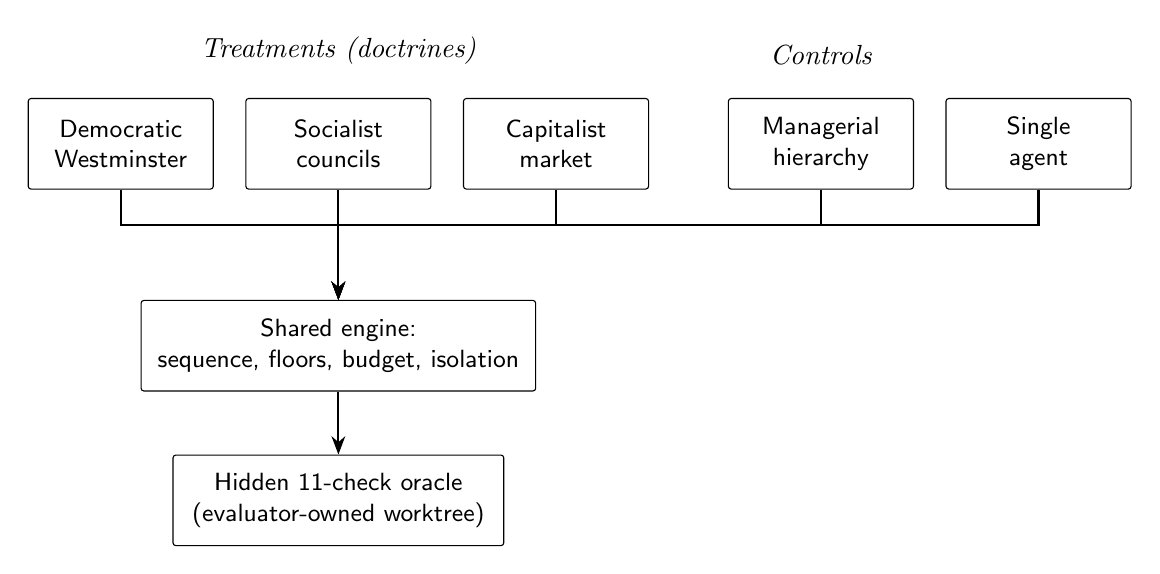
\begin{tikzpicture}[
  font=\small\sffamily,
  box/.style={draw, rounded corners=1pt, align=center, inner sep=6pt, minimum height=1.15cm},
  treat/.style={box, minimum width=2.35cm},
  ctrl/.style={box, minimum width=2.35cm},
  eng/.style={box, minimum width=4.2cm},
  arr/.style={-{Stealth}, thick}
]
\node[treat] (d) {Democratic\\Westminster};
\node[treat, right=4mm of d] (s) {Socialist\\councils};
\node[treat, right=4mm of s] (c) {Capitalist\\market};
\node[ctrl, right=10mm of c] (m) {Managerial\\hierarchy};
\node[ctrl, right=4mm of m] (a) {Single\\agent};

\node[eng, below=14mm of s] (e) {Shared engine:\\sequence, floors, budget, isolation};
\node[eng, below=8mm of e] (o) {Hidden 11-check oracle\\(evaluator-owned worktree)};

\coordinate (treatmid) at ($(d.south)!0.5!(c.south)$);
\coordinate (ctrlmid) at ($(m.south)!0.5!(a.south)$);

\draw[arr] (d.south) -- ++(0,-0.45) -| (e.north);
\draw[arr] (s.south) -- (e.north);
\draw[arr] (c.south) -- ++(0,-0.45) -| (e.north);
\draw[arr] (m.south) -- ++(0,-0.45) -| (e.north);
\draw[arr] (a.south) -- ++(0,-0.45) -| (e.north);
\draw[arr] (e.south) -- (o.north);

\node[above=3mm of s, font=\itshape] {Treatments (doctrines)};
\node[above=3mm of m, font=\itshape] {Controls};
\end{tikzpicture}
}
\caption{Identification layout. Treatments and controls share the engine, budget, task,
and hidden oracle. Doctrine-specific judgement sits above the shared floors, not instead
of them.}
\label{fig:identification}
\end{figure}

The paper's claim is not that democracies, socialist councils, or markets ``win'' at
software, nor that LLM agents are citizens. It is that political institutions can be
written as code with enough fidelity that their characteristic evidence---divisions,
minority reports, returned assignments, bids and escrow---appears in a ledger, and that
this makes institutional form a treatment in a computational experiment. A single
controlled sweep (21~September 2026) is reported as a proof of concept, with the fairness
defects of that sweep disclosed in the results. Repeated trials, not this $N{=}1$ run, are
what would support comparative inference.

Comparative politics already knows how to describe constitutions. What it lacks is a
setting in which those descriptions can be installed, one at a time, as the operating
system of a productive task whose output can be scored without asking a human which
regime they prefer. Language-model agents are a poor substitute for citizens and a
serviceable substitute for boundedly rational clerks: they follow (and invent, and
forget) procedures, they produce a written record, and they can be given identical
instructions under different rules. That is enough for a laboratory. It is not enough
for a theory of democracy.

Three design choices keep the analogy from collapsing into theatre. First, the engine
is doctrine-neutral: sequence and floors do not belong to Westminster, the councils, or
the market. Second, characteristic evidence is specified in advance---divisions,
minority reports, returned assignments, bids---so that a run which does not produce
that evidence has not instantiated the institution, whatever the folder is named.
Third, two non-political controls prevent every contrast from being read as
``democracy versus capitalism.'' If a parliament is slower than a manager, the
comparison is about procedure, not about the Enlightenment.

The rest of the paper proceeds as a methods article. Section~\ref{sec:related} situates
the laboratory in comparative institutional analysis, computational social science, and
multi-agent software. Section~\ref{sec:types} maps the three ideal types and two controls.
Section~\ref{sec:lab} describes the runtime. Section~\ref{sec:design} states the research
design. Section~\ref{sec:results} reports the sweep without overclaiming it.
Section~\ref{sec:discussion} asks what the method offers political science.
Section~\ref{sec:limits} states limitations. Section~\ref{sec:conclusion} concludes.
Appendices separate implemented from essay-only institutions, list the oracle checks, and
give replication commands.

\section{Related work}
\label{sec:related}

\subsection{Institutions as rules, and the problem of isolation}

\citet{north1990} defines institutions as the humanly devised constraints that structure
interaction. \citet{ostrom1990,ostrom2005} supplies the operational counterpart: an
institutional statement names who may do what, under which conditions, with which
sanctions, monitored by whom. The Institutional Analysis and Development (IAD) framework
was built precisely so that rules-in-form could be distinguished from rules-in-use, and
so that action arenas could be compared without assuming that the same noun (``council'',
``market'', ``legislature'') meant the same mechanism.

Comparative research then faced a measurement problem. \citet{lijphart1999} arrays
democracies on executives-parties and federal-unitary dimensions.
\citet{tsebelis1995,tsebelis2002} compresses institutional difference into veto players:
the number, congruence, and cohesion of actors whose agreement is required for policy
change. \citet{cox1997} shows how electoral rules structure strategic coordination.
\citet{martin2011} treats legislative procedure as a coalition-management technology.
These are powerful reductions. They still observe institutions bundled with parties,
voters, and history \citep{pierson2000}. Laboratory experiments isolate treatments in
human subjects \citep{druckman2006,druckman2011}, but they cannot usually install a
Westminster opposition, a recallable coordinating council, and an escrow market as
alternative constitutions for the same productive task.

Political Swarm takes Ostrom's advice literally: write the rules so that an action arena
can be replayed. The cost is analogical. The agents are not citizens; the ``Commons'' is
not a demos; prices are internal bookkeeping. The gain is that allocation, review,
decision thresholds, and non-waivable floors become code paths rather than narratives
about code paths.

\citet{hall1996} distinguish historical, rational-choice, and sociological
institutionalism. The laboratory is closest to the rational-choice branch in one
respect---it treats institutions as constraints on choice---and closest to the historical
branch in another: sequence matters, early refusals constrain later ones, and property
in files is a form of increasing returns \citep{pierson2000}. It is weakest as
sociological institutionalism. There is no culture to socialise into, unless one counts
system prompts, which are too thin to bear that weight. The paper therefore does not
claim to test March and Olsen's logic of appropriateness \citep{march1984}; it tests
whether logics of aggregation, veto, and allocation can be installed as alternative
operating systems for the same task.

That ambition sits beside, rather than inside, field and survey experiment.
\citet{druckman2006,druckman2011} document the growth of experimental political science
as a way to identify causal effects of information, institutions, and elite cues on human
subjects. The present design identifies the effect of \emph{coded} institutions on
\emph{model} subjects. The internal validity target is the same; the population to which
one might generalise is not. Section~\ref{sec:discussion} returns to analogical
inference, which is the only external-validity story this method can honestly tell.

\subsection{Computational social science and agent-based models}

Computational social science has long argued that digital traces and generative models
let researchers study social processes that interviews and aggregate statistics cannot
reach \citep{lazer2009,salganik2018}. Agent-based models are the native method for
``growing'' macros from micros \citep{epstein1996,epstein1999}. \citet{axelrod1984,axelrod1997}
showed that cooperation, culture, and norms can be studied as evolving strategies.
\citet{cederman1997} treated states as emergent rather than assumed actors.

Those models encode institutions as payoff structures, network topologies, or simple
update rules. They rarely encode \emph{procedure}: a Speaker who may not decide the
substantive question; an Opposition that must name a remedy; a second chamber that
revises findings but does not vote on motions; a worker's right to return an assignment;
an assessor forbidden a success fee. Thick procedure is where comparative politics lives.
A laboratory that wants to speak to that literature has to implement offices, not only
incentive parameters.

The distinction is worth labouring. Axelrod's tournaments vary strategies inside a fixed
game \citep{axelrod1984}. Cederman varies agent types inside a geopolitical space
\citep{cederman1997}. Epstein asks whether a macro regularity can be grown from local
rules \citep{epstein1999}. Political Swarm varies the game itself---the offices, the
agenda, the property rule, the price---while holding the ``players'' as constant as a
shared model roster allows. In IAD terms, it treats the action arena as the treatment
and the participants as (noisy) controls \citep{ostrom2005}. That is closer to
constitutional political economy \citep{buchanan1962} than to evolutionary game theory,
even though the implementation happens to use language models.

\subsection{Mechanism design and markets as engineered institutions}

A parallel tradition treats institutions as engineered allocation devices.
\citet{roth2002} describes the economist as engineer: theory, experiment, and computation
in the service of rules that have to work when fielded. \citet{hayek1945} is the knowledge
argument for prices; \citet{coase1937,coase1960} is the argument that firms exist when
internal coordination is cheaper than repeated contracting, and that externalities follow
transaction costs. \citet{olson1965} and \citet{buchanan1962} add the public-goods and
constitutional-calculus problems: shared infrastructure is under-provided, and the rules
for choosing rules are themselves a design object.

The capitalist arm of Political Swarm is an explicit attempt to make that tradition
runnable inside a coding swarm: an exchange, capital accounts, contract shapes, insurance,
and a regulator confined to rights, contract enforcement, and a safety floor. It is not a
model of actually existing capitalism. It is a constitutional market in Roth's sense---a
designed game whose pieces can be inspected.

\subsection{Multi-agent systems, without governance as the treatment}

Classical multi-agent systems already distinguished protocols from agents
\citep{wooldridge2009}. The last three years of LLM swarms have revived that architecture
with linguistic agents. ChatDev organises a virtual software company through a chat chain
\citep{qian2024}. MetaGPT encodes standard operating procedures as meta-programming
\citep{hong2024}. AutoGen supplies a general conversation framework \citep{wu2023}.
Multi-agent debate can improve factuality \citep{du2024}. In all of these systems the
scientific variable is almost always the model, the prompt, the role roster, or the
communication topology.

That is a reasonable engineering research programme. It is not a comparative-politics
research programme. If every swarm is a firm with a CEO, or a pipeline with stages, then
governance is held constant while models vary. Political Swarm inverts the usual
experiment: models, task, and budget are held as constant as the stack allows, and the
decision system is the treatment. The two control arms exist because a Westminster
parliament should be compared not only with councils and markets but with the
organisational forms software engineering already uses.

Debate swarms \citep{du2024} are the nearest neighbour and still not the same object.
They vary whether agents argue; they do not vary whether argument is an Opposition with
a duty to answer, a council minority report, or a priced dispute before an assessor.
The institutional content of disagreement is the variable here. Disagreement as a
prompting trick is not.

\section{Ideal types and their mapping}
\label{sec:types}

The three doctrines are stylized types, not empirical descriptions of the United Kingdom,
the Paris Commune, or any existing market society. Each type is specified in a design
essay and then implemented, only in part, as a \texttt{SwarmStrategy}. Table
\ref{tab:doctrines} summarises the intended mapping along five functions that comparative
institutionalists already use: organisation, allocation, review, decisions, and
accountability. Appendix~\ref{app:implemented} records which of those functions are
actually wired.

\begin{table}[t]
\centering
\small
\caption{Three political doctrines as software institutions. These are mechanisms under
investigation, not claims about real-world regimes.}
\label{tab:doctrines}
\begin{tabular}{@{}p{2.15cm}p{3.55cm}p{3.55cm}p{3.55cm}@{}}
\toprule
Dimension & Democratic & Socialist & Capitalist \\
\midrule
Organisation &
Two chambers, cabinet, shadow cabinet, neutral Speaker &
Worker councils federated by specialist guilds &
Internal task exchange; firms subcontract when cheaper than contracting \\
Allocation &
Committee planning; seats by election, appointment, and lot &
Work by capability, resources by assessed need; right of return &
Competitive bids on comparative advantage \\
Review &
Opposition brief, government reply, constituency division &
Peer review outside authorship; overruled objections preserved &
Assessor with no success fee; court for unsettled disputes \\
Decisions &
Risk-scaled thresholds above a non-waivable constitutional gate &
Subsidiarity, delegate recall, evidence gate &
Priced scarcity, contract shape, regulatory floor \\
Accountability &
Confidence, recall, Question Time, report against the mandate &
Recall, independent diagnosis, commons report &
Profit and loss, insolvency, market report \\
Characteristic evidence &
Divisions, minority reports, Speaker rulings &
Reconnaissance, returned assignments, mutual aid, dissent &
Bids and awards, priced consumption, levies, refused rescues \\
\bottomrule
\end{tabular}
\end{table}

\subsection{Democratic: mixed government as a coding constitution}

The democratic design does not treat democracy as universal voting on every edit. It
follows the mixed-government reading of Westminster: legislature, executive, organised
opposition, committees, a neutral presiding officer, and a professional continuity layer,
under a constitution that binds the majority \citep{bagehot1867,dicey1885,madison1788,montesquieu1748}.
Offices are constituted from the run identifier so that election, appointment, sortition,
rotation, and recall are re-derivable from the ledger. The Speaker screens motions for
admissibility and amends overlapping mandates so that each file has one owner; the office
is barred from striking the last motion on the paper, because a procedural veto of the
entire programme would be a substantive decision. The Opposition must name a remedy that
reaches the next attempt; a standing objection after the House has decided becomes a
minority report rather than a hidden veto. The House of Review sits on findings, not on
motions. Acceptance is a deterministic constitutional gate, independent of ordinary
confidence.

Two further facts matter for interpretation. First, the Commons division is a formula,
not a deliberative sitting: there is no modelled debate on the floor. Second, several
named Westminster pieces---a two-chamber vote on constitutional amendment, a Security
Committee, a working prime minister, Question Time, and an alternative programme---are
nominal or routed to the human (Appendix~\ref{app:implemented}). The arm is a
\emph{partial} operationalization of the essay, which is itself a partial
operationalization of a historical constitution.

Partial is not the same as fake. Sortition for ordinary offices and election for
competence-sensitive ones is an Aristotelian distinction the code actually draws.
Organised opposition with a duty to answer is a Bagehot distinction the code actually
draws. A gate independent of confidence is a Dicey distinction the code actually draws.
What the arm does not draw is a talking Commons. Readers who need floor debate to call
a system a parliament should treat this as a committee-centred Westminster, closer to
\citet{martin2011} than to a C-SPAN feed.

\subsection{Socialist: federation without a managerial class}

The socialist design starts from a question shared across otherwise opposed traditions:
how specialised workers coordinate a common project without letting coordination harden
into a separate class \citep{marx1871,pannekoek1950,cole1920,kropotkin1902}. The recommended
answer is a federated council swarm. Worker councils inspect the repository before the
plan is written. Specialist guilds advise across councils. A coordinating council is
drawn by lot from the run identifier, bounded by mandate, and in principle recallable.
Allocation follows assessed need and subsidiarity; a worker may return an assignment it
cannot take; mutual aid is dispatched only on an actual block. Dissent that loses is
kept. The commons report is filed at the end of finding disposition so that it is built
into the delivery packet.

Again the implementation is thinner than the essay. Recall grounds beyond misallocation
are not enforced; the deciding coordinator is a single persona; planner recall takes
effect on the next run, not this one. What \emph{is} enforced is the production-side
core: reconnaissance, need-weighted assignment, the right of return, mutual aid, minority
reports, and a constitutional gate that will not let correctness be voted into existence.

The right of return deserves emphasis because it is easy to misread as inefficiency.
In a managerial control, a blocked worker is a failed assignment. In the council
doctrine it is a constitutional event: the worker may refuse work it cannot take, mutual
aid may be dispatched, and an independent diagnosis precedes reassignment after repeated
failure. That is closer to \citet{kropotkin1902} than to a retry loop, even when the
implementation is a retry loop with extra records. The records are the institution.

\subsection{Capitalist: a constitutional market, not a free-for-all}

The capitalist design is Hayekian about knowledge and Coasean about the firm, with a
Nozick-like regulator that is supposed to enforce rights rather than plan production
\citep{hayek1945,coase1937,smith1776,friedman1962,schumpeter1942}. Agents bid; awards
favour comparative advantage rather than the strongest absolute bidder; scarce compute is
priced; tightly coupled work may be subcontracted inside a temporary firm; an assessor is
paid without a success fee; escrow releases under a regulatory floor.

The market is constitutional because three commercial parties in agreement still cannot
waive safety, test integrity, or acceptance evidence. It is also incomplete. Public-goods
and venture funds accumulate levies but issue no grants; credit drawn to cover an
insurance-premium shortfall is never repaid; warranty periods are priced but not counted
down; bid-collusion detection is a logged flag, not a block. Those gaps are design facts,
not footnotes to be silently closed in the results narrative.

They are also theoretically informative. \citet{olson1965} predicts that public goods
inside a market will be under-provided unless someone is assigned to supply them. A
treasury that levies but never grants is an unusually pure illustration: the accounting
identity exists, the disbursement function does not. \citet{coase1937} predicts that
firms appear when the cost of using the exchange exceeds the cost of internal
direction; the capitalist arm therefore permits subcontracting rather than forcing every
edit through the auction. Self-dealing is blocked in a single run's register---a firm
may not assess the contract it was paid for---because that conflict is observable
without cross-run history. Collusion among nominally independent bidders is not, and
the runtime refuses to pretend otherwise. Honesty about what a constitution can see is
part of the constitutional design.

\subsection{Controls: hierarchy and the individual}

The managerial control is a conventional software organisation: a roster, capability
scores, a planner, implementers, and a reviewer, without parliament, councils, or
exchange. The single-agent control collapses planning, implementation, and self-review
into one persona. Neither is a political doctrine, and neither is offered through the
user-facing start command. They exist so that any cost of political procedure can be
compared with the organisational forms the rest of the literature already uses. If a
Westminster swarm is slower than a manager, that is a result about procedure, not a
result about ``democracy versus capitalism.''

\section{The laboratory}
\label{sec:lab}

\subsection{Engine versus doctrine}

The runtime makes a constitutional distinction that political theory would recognise as
the difference between the rules of order and the sitting government. The engine owns
\emph{sequence and floors}. It creates an isolated Git worktree, records a baseline,
asks the doctrine to plan and declare ownership, then loops over assignment, execution,
checks, review, decision, and recording. Concurrency is allowed only across tasks with
disjoint declared ownership. After the loop, integration, independent verification,
finding disposition, and doctrine-level acceptance are serial barriers. The engine never
substitutes its judgement for the doctrine's procedure. That boundary is identical in
the three philosophy documents and is traced, mechanism by mechanism, in the
orchestrator contract \citep{carr2026}.

Each doctrine implements the same barrier ports (integrate, verify, dispose,
accept, remediate) with its own offices (Table~\ref{tab:barriers}). Who convenes is
political; that the barriers happen, and in that order, is not.

\subsection{Rules-in-form, rules-in-use, and deterministic offices}

\citet{ostrom2005} insists that rules-in-form and rules-in-use can diverge. The
laboratory makes that divergence inspectable. Some offices are deterministic functions
of the run record: elections and sortition seeded from the run identifier, Commons
divisions computed from a formula, constitutional gates that do not call a model,
assignment returns that ride an implementer dispatch at no extra cost. Running those
offices through an LLM would make them unauditable without making them better. Other
offices weigh evidence and therefore dispatch a model: select committees, Opposition
briefs, government replies, the House of Review, council reconnaissance, mutual aid,
contractual assessment. The pattern implied by the shared orchestrator contract is
simple. A body that applies a rule does not get a model. A body that judges evidence
does.

Two placements are forced by the engine rather than chosen for local colour. The House
of Review sits at finding disposition, not at acceptance, because a second chamber
expressing itself through \texttt{accept()} would hold a veto the doctrine withholds
from it. The socialist commons report is written at the end of disposition rather than
in \texttt{accept()}, because the delivery assembler reads doctrine notes before
acceptance runs; a report filed later would disclose nothing while looking as though it
had. Forced placements are the laboratory equivalent of constitutional conventions
\citep{dicey1885}: they are not in the essay's organisational chart, but violating them
would silently change the constitution.

Run state is similarly constitutional. A swarm may be running, parked on a budget or
human decision, awaiting independent acceptance, completed, in remediation, interrupted,
terminated incomplete, failed, or stopped. Partial work may not be presented as
accepted. Resource exhaustion parks the run; it does not, by itself, end it. Those
distinctions are the difference between a laboratory and a demo.

\begin{table}[t]
\centering
\caption{The same acceptance barriers, three institutions. The engine requires the
ports; the doctrine fills them.}
\label{tab:barriers}
\begin{tabular}{@{}p{2.3cm}p{3.5cm}p{3.5cm}p{3.5cm}@{}}
\toprule
Barrier & Democratic & Socialist & Capitalist \\
\midrule
Integrate &
Integration Committee, answerable to the Commons &
Integration council of producers &
Separately procured integration assessor \\
Verify &
Verifier appointed by the Commons who did not author &
Independent peer outside the authorship chain &
Contractual assessor with no success fee \\
Dispose findings &
Majority report; minority reports preserved &
Common ledger; dissent preserved &
Acceptance schedule with priced obligations \\
Accept &
Constitutional verification gate, then assent &
Recorded acceptance on reproducible evidence &
Escrow release under the regulatory floor \\
Remediate &
Motions recommitted for scrutiny &
Returned to the responsible council &
Warranty claim; repeat failure relists \\
\bottomrule
\end{tabular}
\end{table}

\subsection{Floors as coded vetoes}

\citet{tsebelis2002} treats a constitution as a special veto player: it raises the
threshold for change. Political Swarm encodes two such constraints above every doctrine.
First, no strategy may delete, skip, or weaken an existing test to obtain a pass; the
engine inspects the staged diff before the check runs and opens a human
\texttt{test\_waiver}. Approving the waiver does not land the weakening: it only requeues
the task, and the guard runs again. Second, findings on named grounds---security, safety,
privacy, licensing, human control, test integrity, acceptance evidence---are marked
non-waivable. An ordinary majority, a council vote, or a paid contract cannot
disposition them as accepted without a remedy. Socialist and capitalist strategies call
the same marker as the democratic House of Review. Three constitutions, two prohibitions,
one implementation, so the floors cannot drift apart by doctrine.

This is a stricter analogue of constitutional review than most parliamentary models
use. In \citet{tsebelis2002}, a constitutional court is a veto player whose congruence
with the legislative majority varies. Here the floor is perfectly incongruent with any
doctrine that would like to ship: it is not an agent with preferences, it is a pattern
match plus a prohibition. That is both a strength and a weakness. The strength is
auditability. The weakness is the false positive already noted, and the deeper weakness
that a constitution which cannot learn is closer to a tripwire than to a court. The
laboratory currently offers tripwires. Building a court---an office that interprets the
grounds---would be a different, and more sociological, experiment.

Minority reports are the other floor. A disposition that drops a marked dissent is
restored. Overruled objections remain in the delivery packet. That is an Ostrom-like
monitoring rule: the record of disagreement is part of the common-pool information, not
an embarrassment to be garbage-collected.

\subsection{Packets, isolation, and the human remainder}

Between model instances the engine passes a synchronisation packet: base revision,
decisions, ownership map, changed-file manifest, evidence, open findings. At the end of
a run the doctrine submits a delivery packet: evidence, exact check commands and
results, findings with dispositions, minority reports, limitations, residual risks. The
run reaches \texttt{awaiting\_acceptance}, never \texttt{completed}, on the swarm's own
say-so. An independent check traces every acceptance criterion to evidence, reads the
complete diff, and either completes the run or returns concrete defects to the
\emph{same} swarm. Writes into the user's repository require a further, explicit
confirmation.

This is a laboratory with a sovereign. In live use the sovereign is the human. In the
headless benchmark the user's selected model stands in for doctrine escalations, seeing
the task, the checks, and the diff, and naming no doctrine; budget and wall-clock
extensions are a fixed per-arm allowance. Either way, political procedure does not get
the last word on merging code. That is a feature of the identification strategy, not an
admission that the doctrines failed to be political.

Worktree isolation is a Git boundary, not an operating-system sandbox. Generated commands
are untrusted. The Model Context Protocol cannot cryptographically distinguish a human
request from a model's request to apply. Those are ethical and safety facts, returned to
in Section~\ref{sec:limits}.

\section{Research design}
\label{sec:design}

\subsection{Task}

Every arm receives the same starting repository and the same goal: a small Python command
line program, \texttt{alloydamage}, that computes the neutron displacement-damage
cross-section of an Fe--Cr--Ni alloy from IAEA-traceable elemental data,
\[
\sigma_{d,\mathrm{alloy}}(E)=\sum_{i} x_i\sigma_{d,i}(E),
\]
with documented conversion from weight percent to atomic fraction, a common interpolated
energy grid, no silent extrapolation, CSV and plot outputs, and provenance reachable from
program output. The task is bounded and non-trivial. It requires numerical care,
refusal behaviour, and packaging. It is not a political task. That is the point: the
politics is in the coordination, not in the subject matter.

An engineering task is used for three methodological reasons. First, it yields an
independent, quantitative outcome---the oracle---that does not require a human coder to
prefer one doctrine's style. Second, software work has natural analogues to the
functions in Table~\ref{tab:doctrines}: plans are agendas, files are property, tests are
monitoring, merges are collective decisions. Third, the same task can be given to a
managerial hierarchy and a single agent without changing its meaning, which a
``simulate a parliament'' task could not. The cost is that readers may mistake the paper
for a software-engineering bake-off. The oracle is a measurement instrument, not the
explanandum. The explanandum is whether and how institutional form changes the path to
that measurement.

\subsection{Treatments, controls, and what is held fixed}

The five strategies share the engine, the OpenRouter roster, the per-run budget, and the
task text. Every dispatcher role uses \texttt{openai/gpt-oss-20b} with
\texttt{deepseek/deepseek-v4-flash} as fallback, except the implementer, which uses
\texttt{z-ai/glm-5.2} with the same fallback. The sweep reported below used an eight
dollar budget and a 150-minute wall-clock cap, run sequentially to avoid provider
contention. Strategy order can be rotated across trials; this paper reports one
sequential sweep.

What is \emph{not} held fixed, and should not be, is the number of institutional model
calls. A Speaker ruling, an Opposition brief, council reconnaissance, or a bid round is
the treatment. Equalising call counts would erase the institutions.

The sovereign is the remaining identification threat. Doctrines escalate at different
rates: a Westminster arm can open a vote-threshold or confidence decision; a market arm
can open a spend approval; both can hit the engine's final-diff and test-waiver ports.
In the benchmark, those escalations go to the user's selected model with no doctrine
name and no tools, and the rationale is kept in the evaluator ledger rather than being
fed to the next implementer. Arms that escalate less therefore do not receive a stronger
model's engineering advice as a side payment. Sovereign cost is reported per arm
because it is harness spend, not doctrine spend, and because a constitution that asks
the sovereign more often is a different constitution. Budget and time extensions are a
fixed per-arm allowance, not a first-come pool. Those details are tedious, and they are
the difference between a treatment and a confound.

\subsection{The hidden oracle and blind scoring}

Per-task checks ask a narrow regression question against the latest accepted tree. Final
required checks are strict. Separately, the harness runs an evaluator-owned oracle of
eleven checks against the live worktree before doctrine acceptance (Appendix
\ref{app:oracle}). The swarm never sees the oracle's code or reference data before that
barrier. Failed checks return as findings with origin \texttt{oracle}, equally for every
arm. ``Tests (oracle)'' in the results is this independent count, not the swarm's
self-report.

A two-pass rubric further separates engineering quality from governance process. Pass~1
scores blinded candidate directories on numerical correctness, nuclear-data handling,
tests, documentation, simplicity, plots, and provenance, plus a small resource-efficiency
weight, without strategy names. Pass~2 opens the ledger. The engineering scores are not
to be revised after unblinding. That is a standard experimental hygiene borrowed from
blinded coding studies and from experimental political science's insistence that the
outcome measure not be the treatment \citep{druckman2011}.

\subsection{Prompt neutrality as a design-based check}

A recurring threat in LLM experiments is that the prompt, not the institution, carries
the answer. Earlier Political Swarm sweeps gave the democratic arm task-specific headers,
provenance tokens, and oracle-mirroring checks that the other arms did not receive;
shared layers also leaked alloy-specific text. Those runs are not comparable and are not
reported as evidence here.

A subsequent review found remaining inequalities: the capitalist implementer was told to
write Node.js on a Python task; democratic and single-agent implementers did not see the
whole goal; implementer temperatures differed; sovereign rejection rationales coached
only the arms that escalate; the extension allowance was a first-come pool; democratic
and socialist arms could read memory left by earlier runs. Those defects were removed.
A unit test now fails if any strategy or the dispatcher mentions the benchmark
vocabulary, if an implementer prompt lacks the goal or the shared reminders, if a prompt
names a language or test framework, or if an arm samples its implementer differently.
Knowledge is scoped per run.

The 21~September 2026 sweep still contained several of those inequalities. It is
reported below with that caveat, as a laboratory demonstration, not as a clean estimate
of institutional treatment effects.

\subsection{What would constitute a confirmatory design}

A confirmatory paper would pre-register the five-arm contrast, fix the code at a tagged
commit, run $K$ sequential trials with rotated order, report oracle passes, cost,
duration, completion status, and process traces, and analyse ledgers as event data. This
paper is not that paper. It specifies the laboratory so that that paper can be run.

The smallest honest $K$ is larger than one and smaller than a public-opinion survey.
Language-model output is overdispersed; institutional call sequences are path dependent;
provider congestion is a time-varying confounder. Five to ten sequential trials on a
frozen commit, with rotated order and the neutrality tests green, would support
descriptive contrasts (medians, ranges, characteristic failure modes). Dozens would
still not support a claim about real parliaments. The method's comparative advantage is
mechanism isolation, not sample size in the survey sense.

\section{Results: a proof-of-concept sweep}
\label{sec:results}

Table~\ref{tab:sweep} reports the 21~September 2026 sweep (commit \texttt{1ca47a7}), plus
one democratic re-run after a procedural bug was fixed. Human intervention is coded 1
when the run ended \texttt{terminated\_incomplete} rather than \texttt{completed}---that
is, when bounded remediation stopped short of delivery---and 0 otherwise. Defects are
$11$ minus oracle passes.

\begin{table}[t]
\centering
\caption{One controlled sweep, identical task and roster. Oracle scores are independent
of self-report. The italic row is not part of the sweep.}
\label{tab:sweep}
\begin{tabular}{@{}lrrrrr@{}}
\toprule
Governance & Oracle & Cost (USD) & Time & Incomplete & Defects \\
\midrule
Democratic & 1/11 & 1.56 & 2h10m & 1 & 10 \\
Socialist & 10/11 & 0.48 & 33m & 1 & 1 \\
Capitalist & 10/11 & 1.47 & 1h25m & 1 & 1 \\
Managerial & 11/11 & 0.52 & 29m & 0 & 0 \\
Single-agent & 10/11 & 0.54 & 35m & 1 & 1 \\
\midrule
\textit{Democratic re-run} & \textit{11/11} & \textit{0.66} & \textit{1h03m} & \textit{1} & \textit{0} \\
\bottomrule
\end{tabular}
\end{table}

Three observations are licensed; a fourth is not.

First, the laboratory runs. All five arms produce ledgers, ownership maps, cost traces,
and a worktree that can be oracle-scored. That is the methods result.

Second, institutional form is visible in process, not only in the score. The socialist
arm's characteristic evidence is reconnaissance, returned assignments, and preserved
dissent; it missed the plot check. The capitalist arm's evidence is bids, awards, and
priced consumption; it missed provenance. The single agent missed provenance as well.
Those single misses are exactly the details that earlier, non-neutral prompts had spelled
out---a reminder that coaching had been doing institutional work.

Third, the managerial control completed 11/11 without stopping, cheaper and faster than
the political arms in this sample. On $N{=}1$ that is not a finding that hierarchy
dominates democracy. It is a reminder of why the controls exist. Political procedure has
a call tax. Whether that tax buys review quality is an empirical question for repeated
trials, not a conclusion from one afternoon.

The fourth, unlicensed, observation would be that ``socialism beat democracy.'' It did
not, in any sense this design can support. The democratic 1/11 traces to a generic
procedural defect, not to missing nuclear knowledge. A recommitted committee kept
refusing a motion on the strength of its own earlier refusal, while that motion's checks
passed and the Opposition approved, until attempts ran out (Figure~\ref{fig:stale}).
The abandoned motion owned the program entry point. At the time, the engine could not
hand an abandoned task's files to another task, so the module never ran. Four other
motions were approved and their tests passed. After the stale-refusal loop was fixed,
a re-run scored 11/11 in 63 minutes at \$0.66---and still ended incomplete, because the
doctrine abandoned a nuclear-data motion whose unit tests never passed, even though the
delivered program covered what that motion was for.

\begin{figure}[t]
\centering
% Institutional failure: stale refusal on a recommitted motion.
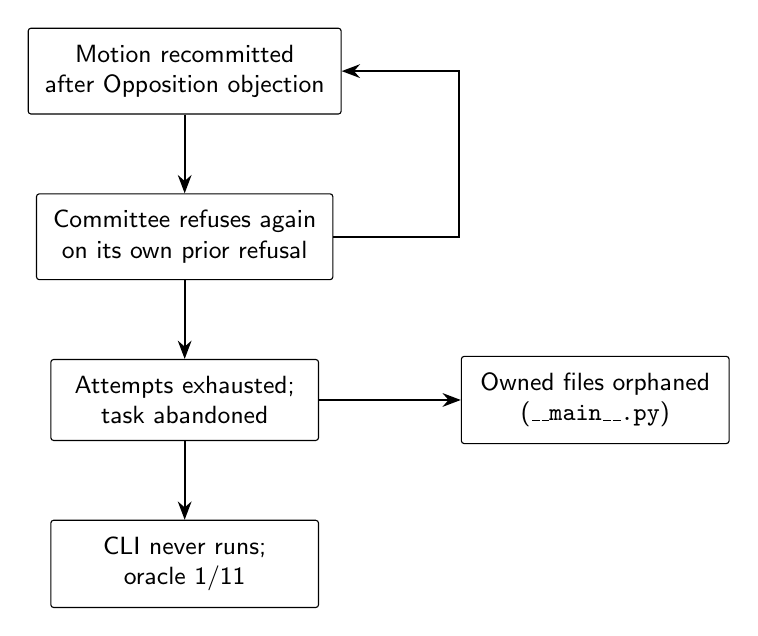
\begin{tikzpicture}[
  font=\small\sffamily,
  n/.style={draw, align=center, inner sep=6pt, rounded corners=1pt, minimum width=3.4cm},
  arr/.style={-{Stealth}, thick}
]
\node[n] (m) {Motion recommitted\\after Opposition objection};
\node[n, below=10mm of m] (c) {Committee refuses again\\on its own prior refusal};
\node[n, below=10mm of c] (a) {Attempts exhausted;\\task abandoned};
\node[n, right=18mm of a] (o) {Owned files orphaned\\(\texttt{\_\_main\_\_.py})};
\node[n, below=10mm of a] (f) {CLI never runs;\\oracle 1/11};

\draw[arr] (m) -- (c);
\draw[arr] (c) -- (a);
\draw[arr] (a) -- (o);
\draw[arr] (a) -- (f);
\draw[arr] (c.east) -- ++(1.6,0) |- (m.east);
\end{tikzpicture}

\caption{Democratic stale-refusal loop on the 21~September 2026 sweep. A committee
treated its own prior refusal as sufficient grounds to refuse again. Agenda cycling
plus exclusive file ownership produced an orphaned entry point and a collapsed oracle
score. The loop is an institutional failure mode, not evidence about democracies.}
\label{fig:stale}
\end{figure}

That sequence is the most politically interesting result in the table, and it is not a
score. It is what \citet{pierson2000} would recognise as a small increasing-returns trap:
an early refusal becomes the reason for the next refusal. It is what
\citet{tsebelis2002} would recognise as a veto player---here, a committee---whose
agreement could not be obtained even after the factual predicate had changed. It is also
what the ownership rule made catastrophic: exclusive property in files, without
succession on abandonment, turned a failed motion into a missing program. Subsequent
engine work transfers orphaned paths to a live task. The political reading is that
property rules and veto rules interact. A methods laboratory that could not produce
that sentence from a ledger would not be worth running.

\subsection{Process traces by arm}

Scores compress. Ledgers do not. On this sweep the socialist arm spent reconnaissance
tokens before the plan existed, which is the point of a council that inspects production
rather than receiving a plan from above. Its single oracle miss was the plot. The
capitalist arm allocated by bid and paid an assessor; its miss was provenance, a public
good in Olson's sense that a market without working grants is liable to under-supply.
The single agent, which has no market and no council, missed provenance too, so the
under-supply is not unique to prices; it is unique to no one owning the public record.
The managerial arm assigned from a roster, reviewed, and finished. It is the cheapest
complete delivery in the table, and the only one that did not stop incomplete.

None of those traces is a regime ranking. They are existence proofs that the
characteristic evidence named in Table~\ref{tab:doctrines} can appear, and that when it
fails to appear---when a Commons does not deliberate, when grants do not disburse---the
paper can say so rather than inferring the missing institution from the name of the
folder.

\section{What the method offers political science}
\label{sec:discussion}

\subsection{Isolable institutions}

The first offering is identification in the IAD sense \citep{ostrom2005}. An action
arena---a coding task with a budget---can be replayed under alternative rule
configurations. The actors' ``preferences'' are noisy and not theoretically clean, but
the rules are inspectable. Comparative statics that are usually cross-national (more veto
players, more delay; more opposition rights, more disclosed risk; more price signals,
different allocation) become within-laboratory contrasts.

Because the rules are code, they can also be ablated. One can disable the Opposition's
duty to name a remedy, or the worker's right of return, or the assessor's ban on success
fees, and ask which piece of the type was load-bearing. That is closer to the way
\citet{ostrom1990} catalogues design principles than to a three-chimaera horse race.
The present paper does not run those ablations. It argues that they are now well-defined
experiments rather than thought experiments.

A related offering is measurement. Institutionalists often infer procedure from
outcomes, or from texts that may not be rules-in-use. Here the ledger is the
rules-in-use. If the Commons does not deliberate, the paper can say so. If grants do
not disburse, the paper can say so. The gap between essay and runtime is not a scandal;
it is data about how much of a historical type survived contact with an engine.

\subsection{Ledgers as process data}

Experimentalists already record choices. Political Swarm records \emph{procedure}:
Speaker rulings, Opposition objections with named remedies, divisions, minority reports,
reconnaissance findings, returned assignments, mutual-aid packets, bids, awards, escrow
releases, refused rescues. Those traces are closer to legislative minutes or to market
microstructure than to a pass/fail. They make it possible to ask not only whether a
constitution delivered, but how it failed: cycling, orphaned ownership, under-provided
public goods, an assessor captured by a success fee (forbidden here by construction).

\subsection{Constitutional floors as coded vetoes}

A large part of constitutional theory is about what majorities must not do
\citep{madison1788,dicey1885,buchanan1962}. Encoding that as a non-waivable finding set,
checked before merge, is a precise analogue of a hard judicial or constitutional
constraint. It is also a warning: the ground patterns are broad, and a false match
(``auth'' inside ``author'') can only be cleared with counter-evidence. Constitutional
text has the same problem. The laboratory makes the false-positive visible.

\subsection{Mixed government, knowledge, and recall}

The three doctrines reconstruct three classic answers to the coordination problem.
Westminster mixed government separates proposal, execution, scrutiny, and adjudication
\citep{bagehot1867,montesquieu1748}. Council socialism tries to keep coordination
recallable so that it does not become a class \citep{marx1871,pannekoek1950}. Markets
treat knowledge as dispersed and use prices and contract rather than a planner
\citep{hayek1945,coase1937}. Running them on one engine does not adjudicate those
traditions. It shows that each answer can be made into a protocol with characteristic
failure modes. That is closer to what \citet{epstein1999} asked of generative models---can
you grow the phenomenon?---than to a horse race.

\subsection{What the method cannot claim}

LLM agents do not have interests, constituencies, or legitimacy. There is no preference
aggregation theorem here, and no welfare comparison. External validity to human
legislatures, firms, or movements is not on offer. The analogy is institutional, not
ontological: these are \emph{as-if} parliaments, councils, and markets. Treating a
cheap model failing a nuclear-data parser as evidence about socialism would be a category
error the laboratory is designed to make obvious.

Analogical inference, used carefully, is still inference. If exclusive file ownership
plus an unreformed veto produces orphaned work, one has a mechanism that
\emph{could} operate wherever property in agenda items is exclusive and succession on
abandonment is undefined. If a treasury levies for public goods and never spends, one
has a mechanism that could operate wherever earmarks exist without a disbursement rule.
Those are statements about coded institutions, offered to theorists of human institutions
as hypotheses, not as results about humans. \citet{greif2006} studies historical
institutions with a similar division of labour: the model is not the city; it is a claim
about a mechanism the city might have used.

A second boundary is welfare. Nothing in the oracle is a social-welfare function.
Managerial 11/11 is not ``hierarchy is just.'' Democratic incompleteness is not
``gridlock is illegitimate.'' The only normative commitment in the runtime is the set of
non-waivable grounds, and those are safety engineering, not political philosophy, even
when they are written in constitutional vocabulary.

\section{Limitations and ethics}
\label{sec:limits}

The empirical limitations are severe and should govern citation. One sweep is one draw
from a nondeterministic process. The reported sweep was not fully prompt-neutral. Several
essay institutions are unwired (Appendix~\ref{app:implemented}). Doctrines differ in
institutional call volume by design, which confounds ``governance'' with ``more
reviewers'' unless process evidence is read alongside scores. OpenRouter availability
and pricing are external. Verification categories are repository-configured.

The ethical limitations are structural. Worktrees isolate Git history; they do not
sandbox the network or the filesystem. Apply protection is procedural. Humans remain
mandatory reviewers of untrusted code. Benchmark spend is real money. The live dashboard
can display historical propaganda images; they are not used in this paper and are not
part of the identification strategy.

A subtler ethical issue is anthropomorphism. Naming a function \texttt{Speaker} does not
create a legislature. The prose in this paper uses institutional names because the code
does, and then immediately qualifies them as stylized types. Readers who skip the
qualifiers will over-read. That is a communication risk the project accepts by choosing
political vocabulary at all.

There is also a research-ethics point about evaluation. Hidden oracles and blinded
scoring are good design. They are not licences to treat model labour as costless or to
hide the dollar cost of a sweep. The table reports spend because spend is part of the
institutional tax. A doctrine that ``wins'' by exhausting a budget another doctrine did
not get was not compared. The 22~September fairness fixes exist because that comparison
had not been clean.

\section{Conclusion}
\label{sec:conclusion}

Political science has better theories of institutions than it has laboratories in which
those theories can be installed as alternative operating systems for the same task.
Political Swarm is one such laboratory: three political doctrines and two controls, a
shared engine, non-waivable floors, a hidden oracle, and a ledger that records procedure
rather than only product. The 21~September 2026 sweep shows that the laboratory functions
and that institutional bugs are scientifically informative. It does not rank regimes.

The replication path is the repository. A tagged engine, an identical starting task, a
fixed roster and budget, sequential execution, the eleven-check oracle, and the two-pass
rubric are enough to turn this methods paper into a results paper---provided the
neutrality tests stay green and $N$ is no longer one. Until then, the honest claim is
narrower, and sufficient: institutions can be written as code, and when they are, they
can be compared.

That claim is addressed to two audiences who do not usually share a methods section.
Computational social scientists already run agents; they have not usually run
constitutions. Comparativists already theorise constitutions; they have not usually been
able to install them. If the laboratory is useful, it will be because those two
literatures can argue, in the same table, about whether a Speaker who cannot strike the
last motion, a council that may return work, and a market that cannot waive a safety
floor are different enough to matter. The argument will have to be about ledgers, not
about which political vocabulary one finds congenial.

\appendix
\section{Implemented versus essay-only institutions}
\label{app:implemented}

Claims in the main text about ``how the institution works'' are restricted to mechanisms
that the orchestrator contract and strategy modules actually run. The design essays are
statements of intent. Table~\ref{tab:gaps} lists the gaps decided as disclosed-not-built
on 22~September 2026, plus related known limitations. The implementation-status note after
the table records subsequent changes; the empirical results in this paper predate them.

\begin{table}[h]
\centering
\caption{Essay institutions that do not run, or do not run as the essay describes.}
\label{tab:gaps}
\begin{tabular}{@{}lp{10.2cm}@{}}
\toprule
Doctrine & Gap \\
\midrule
Democratic &
Two-chamber vote: \texttt{constitutional\_amendment} computes two-thirds of the Commons
as advice and always goes to a human. The House of Review never votes on a motion. \\
Democratic &
No Security Committee. \texttt{security\_boundary} is advice plus a high-severity
Opposition objection, then a human. \\
Democratic &
Commons division is a formula without floor deliberation. Prime minister, Question Time,
and alternative programme were nominal in the measured version. \\
Socialist &
Recall grounds beyond misallocation are not enforced. Lost confidence, concealed
evidence, and council recall of the coordinator are unimplemented. \\
Socialist &
The deciding coordinator was one persona. Planner recall took effect on the next run. \\
Capitalist &
Public-goods and venture funds accumulate levies but issue no grants. \\
Capitalist &
Credit is never repaid. Warranty periods are not counted down; chargeback is not
enforced. Retention may be forfeited although it was never credited. \\
Capitalist &
Bid-collusion detection is informational. Arbitration rarely changes outcomes. \\
Controls &
Managerial and single-agent risk class is recorded, not acted on. \\
\bottomrule
\end{tabular}
\end{table}

Mechanisms that \emph{are} wired, and that therefore license the main-text narrative,
include: democratic office constitution from the run identifier; Speaker screening and
mandate amendment; Opposition review with a required remedy; formulaic Commons votes;
House of Review on findings; minority-report restoration; socialist reconnaissance,
subsidiarity routing, assignment return, mutual aid, dissent preservation, and the
commons report; capitalist bidding and award scoring, capital accounts, contractual
assessment, antitrust self-dealing blocks, and the shared non-waivable floor.

\paragraph{Implementation status after the measured version (28 September 2026).}
The working tree now records versioned decisions and revocable mandates; equal
constituency ballots elect the Prime Coordinator, virtual constituents elect Commons
representatives, and expressed representative Commons and confidence ballots can
decide motions or replace the executive. A defeated motion's Opposition repair proposal
receives a separate amendment ballot. Constitutional motions need two-thirds support
in both Commons and House of Review; security-boundary motions need a separate
Security Committee ballot before the human and safety gates.
Work-council members ratify a plan before assignment, and a diagnosed specification
failure can recall the planner and revise unfinished work within the same run. Members
can initiate a separate delegate-recall ballot for concealed evidence or lost confidence.
Need-weighted task reservations, contract-specific escrow lots, credit repayment, named public-good
grants and exploratory prototype grants with renewed bidding, and supplier delivery
deadlines now have runtime paths. Experiment findings are recorded even on failure.
Outcome contracts and tournaments are unavailable without evaluator baselines and
isolated candidate worktrees. Independent latent-defect attribution and post-run
warranty processing remain unimplemented. Benchmark output now counts mechanism activations, but no new paid
paired trials support an outcome claim about these changes.

\section{Oracle checks and scoring}
\label{app:oracle}

The evaluator-owned oracle (\texttt{benchmark/oracle/checks.py}) runs eleven checks:

\begin{enumerate}
\setlength{\itemsep}{0.15em}
\item Pure-Fe reproduction against the elemental curve.
\item Fifty-fifty atomic Fe--Ni mixture equals the arithmetic mean.
\item Weight-percent to atomic-fraction conversion.
\item Composition normalisation.
\item Unsupported element flagged, not silently filled.
\item Interpolation accuracy on a synthetic grid.
\item No extrapolation beyond native data range.
\item CSV schema and values.
\item Plot generation (PNG above a minimum size).
\item Logarithmic neutron-energy axis.
\item Provenance reachable from program output.
\end{enumerate}

Pass~1 of the scoring rubric weights numerical correctness 30 percent, nuclear-data
handling 20 percent, verification 15 percent, documentation 10 percent, simplicity 10
percent, plots 5 percent, provenance 5 percent, and resource efficiency 5 percent, and
is conducted on anonymized candidate directories. Pass~2 joins strategy names and ledger
process evidence without revising Pass~1.

\section{Replication}
\label{app:replication}

The laboratory is the public repository \url{https://github.com/dgcarr/political-swarm}
(Apache License 2.0). From \texttt{mcp-server/}, with an OpenRouter key configured:

\begin{verbatim}
npm run benchmark -- --label controlled-run \
  --budget-usd 8 --max-wall-clock-min 150
\end{verbatim}

This invokes real models and costs money. Use identical configuration, task commit,
budget, environment, and scoring for every strategy. Resume an interrupted sweep with
\texttt{--resume}. Sequential execution is the comparison mode; \texttt{--concurrent} is
stress only. Compile this paper with \texttt{pdflatex}, \texttt{bibtex}, and two further
\texttt{pdflatex} passes in \texttt{papers/institutions-as-code/}.

\bibliographystyle{apalike}
\bibliography{references}

\end{document}
